\documentclass[tikz,border=10pt]{standalone}
\usetikzlibrary{shapes,arrows,positioning,calc,fit}

\begin{document}

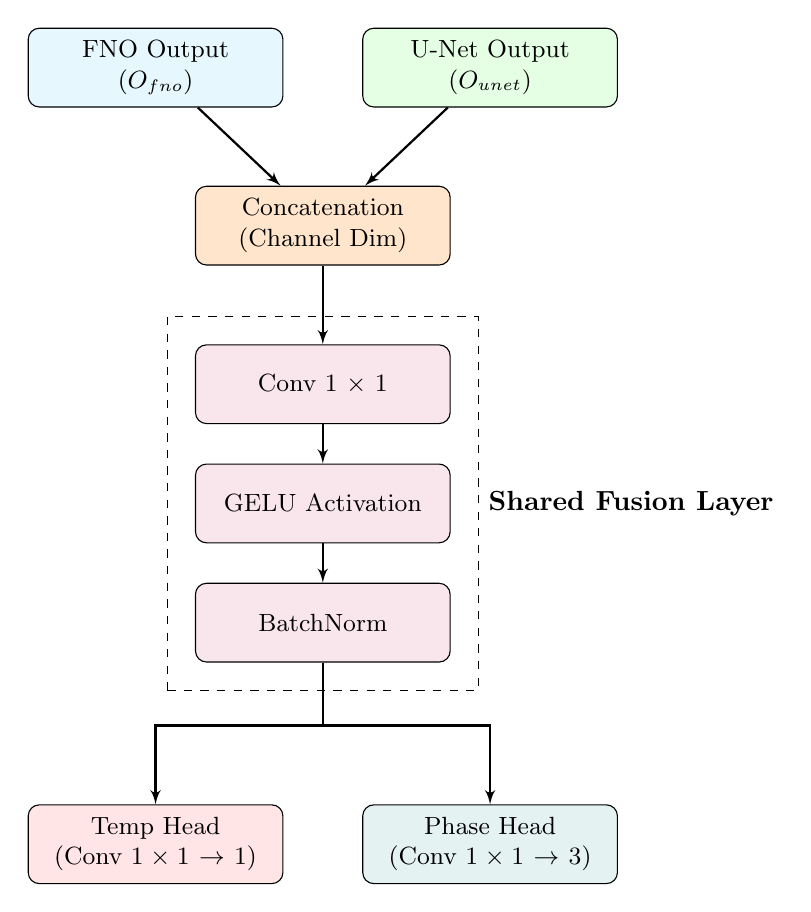
\begin{tikzpicture}[
    node distance=1.0cm,
    auto,
    block/.style={
        rectangle, 
        draw, 
        fill=blue!10, 
        text width=3cm, 
        text centered, 
        rounded corners, 
        minimum height=1cm,
        font=\small
    },
    op/.style={
        circle,
        draw,
        fill=yellow!20,
        inner sep=2pt,
        font=\small\bfseries
    },
    line/.style={
        draw, 
        -latex', 
        thick
    }
]

    % Inputs
    \node [block, fill=cyan!10] (fno_out) {FNO Output\\($O_{fno}$)};
    \node [block, fill=green!10, right=1cm of fno_out] (unet_out) {U-Net Output\\($O_{unet}$)};
    
    % Concat
    \node [block, fill=orange!20, below=1.5cm of $(fno_out)!0.5!(unet_out)$] (concat) {Concatenation\\(Channel Dim)};
    
    % Shared Layers
    \node [block, fill=purple!10, below=1cm of concat] (conv) {Conv $1\times1$};
    \node [block, fill=purple!10, below=0.5cm of conv] (gelu) {GELU Activation};
    \node [block, fill=purple!10, below=0.5cm of gelu] (bn) {BatchNorm};
    
    % Grouping Shared Layers
    \node [draw, dashed, inner sep=10pt, fit=(conv) (gelu) (bn), label=right:\textbf{Shared Fusion Layer}] (shared) {};
    
    % Split
    \coordinate [below=0.8cm of bn] (split);
    
    % Heads
    \node [block, fill=red!10, below left=1cm and 0.5cm of split] (head_temp) {Temp Head\\(Conv $1\times1 \to 1$)};
    \node [block, fill=teal!10, below right=1cm and 0.5cm of split] (head_phase) {Phase Head\\(Conv $1\times1 \to 3$)};
    
    % Edges
    \path [line] (fno_out) -- (concat);
    \path [line] (unet_out) -- (concat);
    
    \path [line] (concat) -- (conv);
    \path [line] (conv) -- (gelu);
    \path [line] (gelu) -- (bn);
    \path [line] (bn) -- (split) -| (head_temp);
    \path [line] (bn) -- (split) -| (head_phase);

\end{tikzpicture}

\end{document}
